\newpage
\section{Реализация}

% Если в рамках работы проводится реализация некоторого программного средства,
% то в разделе «Описание практической части» обязательно должна быть описана
% его программная реализация, в частности:
% приведены обоснования выбранного инструментария;
% приведена с иллюстрацией общая архитектура разработанного средства;
% приведена с иллюстрацией схема работы средства;
% если осуществляется доработка существующего средства, то должны быть описаны
% новые возможности/улучшения, реализованные в данной работе.
% обязательно должны быть приведены характеристики функционирования (например,
% сложность, производительность, время реакции и т.д.)
\subsection{Библиотека libsvm}
Предложенный в разделе \ref{research} метод использует в своей работе метод опорных вектров. Этот метод используется во многих задачах и поэтому существует некоторое количество открытых реализаций метода. Одной из самых известных является библиотека libsvm\cite{LIBSVM}.
Библиотека libsvm содержит реализацию метода опорных векторов. Она содержит интерфейсы для построения моделей по обучающей выборки и предсказания значения целевой функции по  существующей модели. Дополнительно эта библиотека содержит интерфейсы для сохранения модели в файл и загрузки ее из файла.

Для создания модели можно пользоваться несколькими ядровыми функциями(линейная, полиномиальная, сигмоид и другие), а также задавать все необходимые для работы метода параметры.

Кроме того можно указывать тип решаемой задачи: классификация, классификация с двумя классами, регрессия и др.
Так как libsvm имеет интерфейс для ее использования из языка C(это необходимо для ее использования в dspam), а также распространяется под свободной лицензией, она была использована при реализации разработанного метода.

%Существует\cite{GPUSVM} версия библиотеки libsvm использующая современные графические процессоры, логика работы в которой написана на CUDA. Использование графических процессоров позволяет существенно уменьшить время построения модели и время предсказания(смотри график \ref{CUDASVM}).

%\begin{figure}[h]
%\begin{center}
%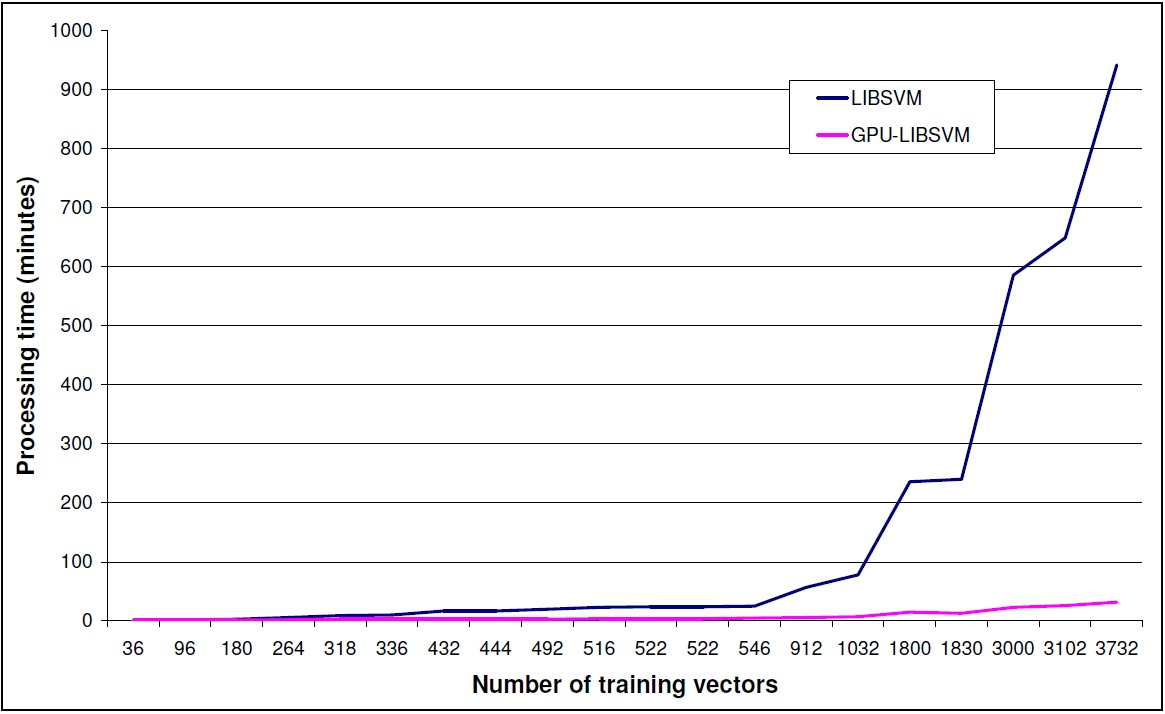
\includegraphics[width=10cm]{img/GPULIBSVM-comparison}
%\end{center}
%\caption{Сравнение производительности обычной версии libsvm и libsvm с использованием CUDA}
%\label{CUDASVM}
%\end{figure}

%Вместе с библиотекой поставляются некоторое количество исполняемых файлов, которые позволяют строить модель по данным из файла в определенном формате, а также осущесвлять предсказание для даннах записанных в файле по построенноей модели. Также поставляется некоторое количество тестовых данных.

\subsection{Архитектура dspam}
В основе dspam лежит библиотека libdspam, которая реализует логику фильтрации.
Эта библиотека содержит код нескольких алгоритмов фильтрации (одновременно использоваться может только один из них)
Кроме того библиотека содержит несколько вспомогательных классов реализующих некоторые структуры данных(списки, деревеья и т. п), а также драйвер хранилища данных.

Данные могут храниться либо в одной из поддерживаемых СУБД(это MySQL, Posgres и SQLite), а также непосредтсвенно в файловой системе(используется собственная методика хранения пар ключ-значение).

\begin{figure}[h]
\begin{center}
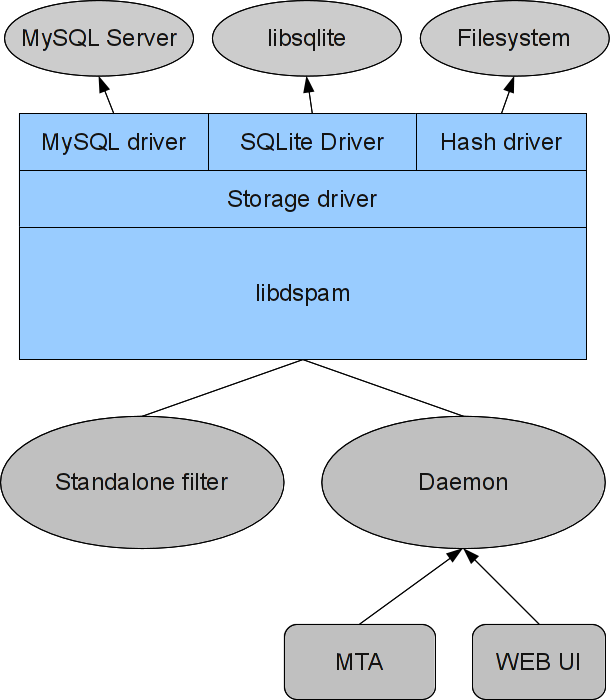
\includegraphics[width=10cm]{img/dspamarch}
\end{center}
\caption{Архитектура dspam}
\label{dspamarch}
\end{figure}

Dspam может работать либо в режиме standalone-фильтра, либо демона. В обоих случаях
исполняемый модуль линкуется с библиотекой libdspam.

Работа в standalone режиме подразумевает что бинарный файл запускается по требованию. Тестируемое письмо в этом случае подается исполняемому модулю на стандартный вход, а информацию о произведенном тестировании можно
получить со стандартного вывода. Эта информации может быть представлена в виде короткой строчки в которой содержится класс, к которому отнес классификатор письмо и вероятностью или в виде самого письма с установленными заголовками. Этот режим удобно использовать для тестирования системы, а так же в случае кода количество писем достаточно мало и требование к производительности невелики.

Работа в режиме демона подразумевает что исполняемый код постоянно находится в оперативной памяти. Общение с клиентом в этом случае происходит либо через сеть (используется tcp-сокет), либо через UNIX-сокет. Таким образом dspam в этом случае является полноценным серверным приложением. Сервер по запросу от клиента принимает письмо, классифицирует, проставляет необходимые заголовки и возвращает клиенту. Клиентом в таком случае выступает система доставки почты(MTA).

Кроме того сервер может выполнять некоторые сервисные команды: просмотр статистики, очистка хранилища данных и т. п. В этом случае клиентом может быть например web-интерфейс администратора.


\subsection{Описание реализации}
	Для обеспечения работы описанного в разделе\ref{research} метода были произведены следующие действия:
\begin{enumerate}
\item В библиотеку dspam добавлен модуль, отвечающий за добавление письма в обучающую выборку метода опорных векторов. Работает с письмами, уже разбитыми на лексемы. Записывает в специальный файл информацию об адресате письма и частотах лексем.
\item Разработана программа на языке python, определяющая частоты каких лексем будут использоваться в качестве признаков методом опорных векторов, подготавливающая данные для инструмента svm-train из комплекта библиотеки libsvm и вызывает этот инструмент, который строит модель для метода опорных векторов. Эта программа также генерирует файл с описанием модели, используемый в дальнейшем при классификации. Программу необходимо вызывать каждый раз при необходимости перегенерации модели(например можно ее вызывать каждые сутки при помощи стандартной службы CRON).  
\item В библиотку dspam добавлена функциональность, позволяющая произвести классификацию письма по модели ии ее описанию. По описаню модели и самому письму строится векторное представление письма, затем при помощи библиотеки libsvm по модели и вектору получается оценка принадлежности письма одному из классов.
\end{enumerate}

\subsection{Схема работы}
Опишем схему работы разработанного средства в различных случаях.
Всего есть три стадии работы системы:
\begin{itemize}
\item \textbf{Добавление письма в обучающую выборку}. Реализуется при помощи функциональности, содержащейся в libdspam.
\item \textbf{Построение модели}. Реализуется внешней программой, вызываемой по требованию.
\item \textbf{Классификация}. Реализуется при помощи функциональности содержащейся в libdspam и libsvm.
\end{itemize}

Опишем подробно что происходит на каждом из этапов.

\begin{figure}[h]
\begin{center}
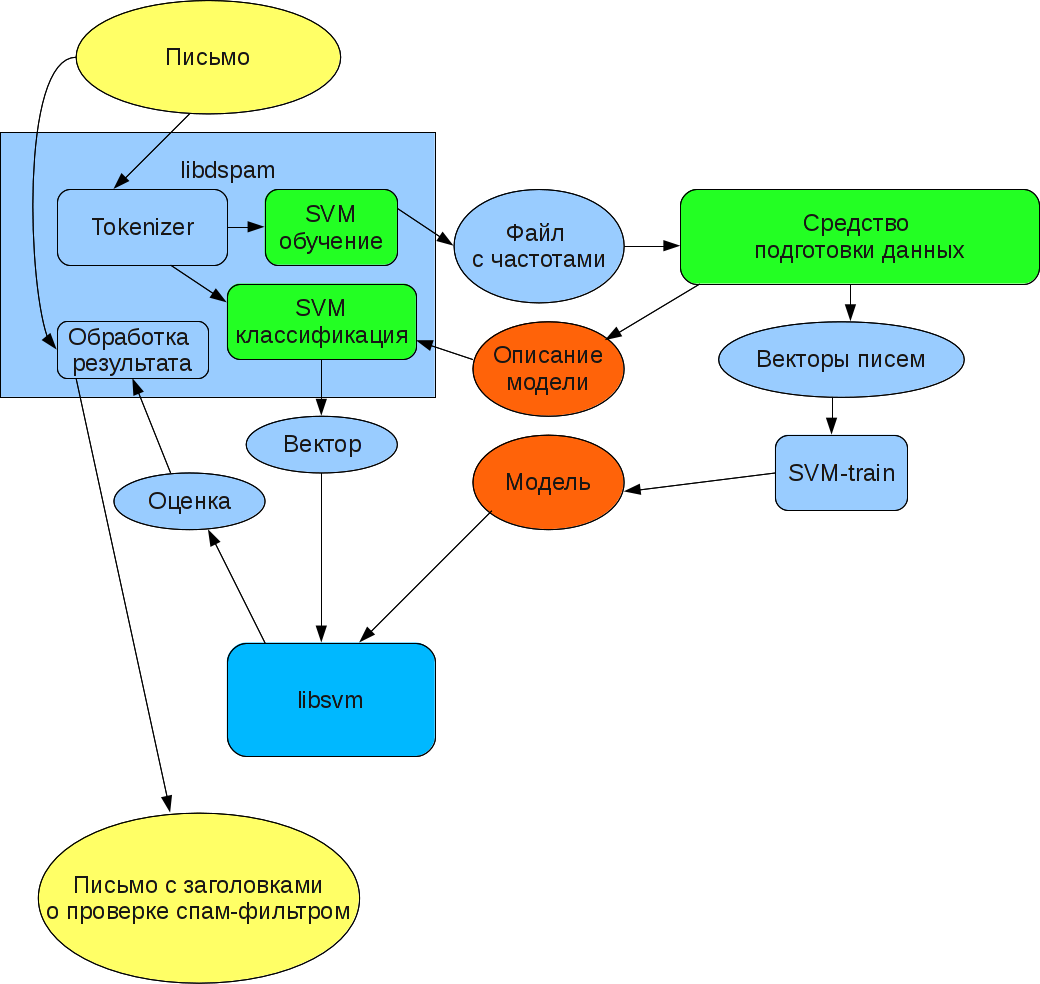
\includegraphics[width=12cm]{img/working_scheme2}
\end{center}
Зеленым выделенны компоненты, реализованные в рамках работы\caption{Cхема работы классификатора. Зеленым выделенны компоненты, реализованные в рамках работы}
\label{dspamarch}
\end{figure}

\subsubsection{Добавление письма в обучающую выборку}

\begin{enumerate}
    \item Письмо попадает в систему.
    \item Письмо разбивается на лексем.
    \item Вычисляются частоты лексем.
    \item Информация о классе письма, адресате и частотах лексем записывается в файл частот.
\end{enumerate}

\subsubsection{Построение модели}
\begin{enumerate}
    \item Вызывается скрипт построения модели (вызов происходит раз в день при помощи стандартной службы CRON).
    \item Вычисляются общие частоты лексем для каждой лексемы из файла частот.
    \item Выбираются наиболее употребимые лексемы (лексемы с наибольшей частотой).
    \item Для каждого из писем строится вектор, содержащий частоты наиболее употребимых лексемы, а также индикаторы принадлежности письма пользователю (все кроме одного индикаторы равны нолю).
    \item Построенное множество векторов записывается во временный файл вместе с информацией о классах писем,  соответсвующих векторам.
    \item По построенному временному файлу генерируется модель при помощи инструмента svm-train.
    \item Информация о лексемах используемых для построения модели сохраняется во временный файл описания модели.
\end{enumerate}

\subsection{Классификация}
\begin{enumerate}
    \item Письмо попадает в систему.
    \item Выясняется адресат письма.
    \item Письмо разбивается на лексемы.
    \item Вычисляются частоты лексем.
    \item Загружается описание модели
    \item По описанию модели, адресату и частотах лексем строится вектор
    \item Загружается модель
    \item По модели и вектору вычисляется вероятность принадлежности письма спаму
    \item По пороговому правилу выставляется оценка спам/не спам
\end{enumerate}

